\documentclass[11pt]{book}
\usepackage{geometry}        
\geometry{letterpaper}    
\usepackage[parfill]{parskip}  
\usepackage{graphicx}
\usepackage{amssymb}
\usepackage{epstopdf}

\DeclareGraphicsRule{.tif}{png}{.png}{`convert #1 `dirname #1`/`basename #1 .tif`.png}

\usepackage[colorlinks=true, pdfstartview=FitV, linkcolor=blue, 
            citecolor=blue, urlcolor=blue]{hyperref}

%\includeonly{Chapter1}
\usepackage{geometry}                		% See geometry.pdf to learn the layout options. There are lots.
\geometry{letterpaper}    
\usepackage{graphicx}
  \usepackage{ams math}
  \usepackage{tikz}
 \usepackage{tcolorbox}
 \tcbuselibrary{skins}
 \tcbuselibrary{theorems}
\usepackage{hyperref}   
\usepackage{color}
\newcommand{\VAR}{CTRL-r }
%\usepackage[dvipsnames]{xcolor}
         		% ... or a4paper or a5paper or ... 
%\geometry{landscape}                		% Activate for for rotated page geometry
%\usepackage[parfill]{parskip}    		% Activate to begin paragraphs with an empty line rather than an indent
\usepackage{graphicx}				% Use pdf, png, jpg, or eps§ with pdflatex; use eps in DVI mode
								% TeX will automatically convert eps --> pdf in pdflatex		
\usepackage{amssymb}


%\author{The Author}
%\date{}							% Activate to display a given date or no date
%\newcommand{\inp}[1]{\texttt{\colorbox{yellow!25}{#1}}}
\newcommand{\inp}[1]{\begin{tcolorbox}[colback=yellow!25!,colframe=black]\texttt{#1} \end{tcolorbox}}

%\newcommand{\proc}[1]{\texttt{\colorbox{green!25}{#1}}}
\newcommand{\proc}[1]{\begin{tcolorbox}[colback=green!35!white,colframe=black]#1 \end{tcolorbox}}
 
 \newcommand{\coqtwo}[2]{
 \begin{tcolorbox}[bicolor,righthand width=\linewidth/4,sidebyside,colback=green!35!white,colbacklower=gray!10!white] {\small \texttt{#1}}\tcblower
$#2$ \end{tcolorbox}}
 
\newcommand{\coq}[1]{\begin{tcolorbox}[colback=gray!10!white,colframe=black]$#1$ \end{tcolorbox}}
\newcommand{\mess}[1]{\begin{tcolorbox}[colback=white,colframe=black] #1 \end{tcolorbox}}
\newtheorem{Theorem}{Theorem}
\newtheorem{Lemma}{Lemma}
\newtheorem{Proposition}{Proposition}
\newtheorem{Definition}{Definition}
\newtheorem{Axiom}{Axiom}
\tcbuselibrary{breakable}


\newtheorem{theorem}{Theorem}
\newtheorem{corollary}[theorem]{Corollary}
\newtheorem{definition}{Definition}
\newtheorem{lemma}{Lemma}
\newtheorem{exercise}{Exercise}
\newtheorem{remark}{Remark}
\newtheorem{example}{Example}
\newtheorem{warning}{Warning}

\def\grad{ \mbox{grad}}
\def\curl{ \mbox{curl}}
\def\div{ \mbox{div}}
\def\U{\ensuremath {\cal U}}
\def\S{\ensuremath {\cal S}}
\def\V{\ensuremath {\cal V}}
\def\R{\ensuremath {\cal R}}
\def\tr{\ensuremath {\mbox{tr}}}




% ------------------- Title and Author -----------------------------
\title{Sample Book}
\author{Author}
\begin{document}


\frontmatter
\maketitle

\tableofcontents


\section{ Installation}

\subsection{Mac OSX}
\begin{enumerate}
\item Download and install  the latest version of Coq (it needs to be at least 8.6) from :

\href{https://coq.inria.fr/download}{https://coq.inria.fr/download}

Move it to your apps folder.


\item  Download and unpack spatchocq.app from canvas
move the spatchcoq.app to Applications and start it. 

\item when prompted find the Coq installation you have just move above. Navigate to 
\begin{verbatim}
/Applications/CoqIDE_8.6.app/Contents/Resources/bin/
\end{verbatim}
and choose coqtop. See Figure~\ref{fig:macos}

You only do this once.
\item  You only have to do this once. You might also need to install gtk, the simplest way to do this is  via homebrew
{\center brew install gtk+}
\begin{figure}\label{fig:macos}
\center
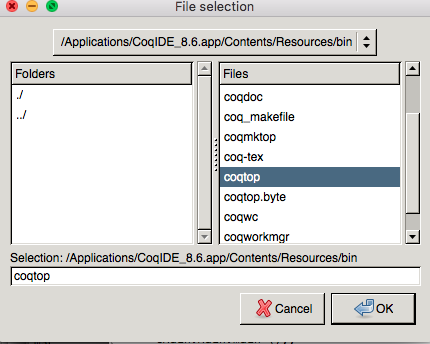
\includegraphics[scale=0.5]{Installation/macos.png}
\caption{Choose the Coq app in a Mac env}\label{fig:macos}
\end{figure}
\item enjoy

\end{enumerate}

\subsection{Windows}
\begin{enumerate}

\item get the zipfile spatchcoq.zip,  unzip it in a folder on a usb stick and doubleclick the application file spatchcoq. 
Note this version includes an instalation of Coq (not very extensively tested yet)

\item enjoy
\end{enumerate}


\subsection{Linux}
\begin{enumerate}
\item Download and install  the latest version of Coq it needs to be at least 8.6 so do not use 
apt-get install coq
\item  go to https://github.com/corneliuhoffman/spatchcoqocaml/tree/master
to build from scratch.
\item when prompted go to the Coq folder you just installed with opam and find  the application called {\bf coqtop}

\item enjoy
\end{enumerate}











\part{ Description of the tactics and hints}
\chapter{Tactics}

\section{This is trivial.}

This will only work on very easy statements. If it works it will solve the current goal. Try to avoid overuse. Do better than your lecturers.


\section{I cannot prove this.}

If you are stuck this tactic will ``prove'' the current goal. If you use this in a proof at the end if the proof when you try to use Qed you will get the following error
\mess{``Error:Attempt to save a proof with given up goals. If this is really what
you want to do, use Admitted in place of Qed.}
To avoid the error just type Admitted instead of Qed.


\section{Prove left hand side.}
Suppose you want to prove the following goal:
\coq{\cdots\\ 
===== \\ 
P\lor Q}

The above mentioned tactic will the produce a the following goal

\coq{\cdots\\ 
===== \\ 
P}
 and so you will have to now prove a simple goal.

\section{Prove right hand side.}
Symmetric with the above, suppose you want to prove the following goal:
\coq{\cdots\\ 
===== \\ 
P\lor Q}

The above mentioned tactic will the produce a the following goal

\coq{\cdots\\ 
===== \\ 
Q}



\section{Prove VAR in the disjunction.}
This tactic combines the above two. More precisely,
suppose you want to prove the following goal:
\coq{\cdots\\ 
===== \\ 
P\lor Q}

Then applying 
\inp{Prove P in the disjunction.}

will produce the goal 
\coq{\cdots\\ 
===== \\ 
P}
while applying
\inp{Prove Q in the disjunction.}

will produce the goal 
\coq{\cdots\\ 
===== \\ 
Q}

\section{Eliminate the conjuction in hypothesis VAR.}

Suppose your goal looks like
\coq{\cdots\\ 
Hyp: P\land Q\\
\cdots \\
===== \\ 
\cdots}

Then applying 
\inp{Eliminate the conjunction in hypothesis Hyp.}
will produce a goal similar to the one below:

\coq{\cdots\\ 
Hyp: P\\
Hyp0: Q\\
\cdots\\
===== \\ 
\cdots}
allowing you to use the parts of Hyp independently.


\section{Consider cases based on disjunction in hypothesis VAR.}
Suppose your goal looks like
\coq{\cdots\\ 
Hyp: P\lor Q\\
\cdots \\
===== \\ 
\cdots}
Then applying 
\inp{Consider cases based on disjunction in hypothesis Hyp.}
will produce two separate goals similar to the one below:
\coq{\cdots\\ 
Hyp: P\\
\cdots \\
===== \\ 
\cdots}

\coq{\cdots\\ 
Hyp: Q\\
\cdots \\
===== \\ 
\cdots}

obtaining a proof by cases.

\section{Prove the conjunction in the goal by first proving VAR then VAR.}
Suppose your goal looks like
\coq{\cdots\\ 
===== \\ 
P\land Q}
 Then 
 \inp{Prove the conjunction in the goal by first proving P then Q.}
 
 will separate the proof in two different goals
 
 \coq{\cdots\\ 
===== \\ 
P}
\coq{\cdots\\ 
===== \\ 
Q}

 
\section{Assume VAR then prove VAR.}
Suppose your goal looks like
\coq{\cdots\\ 
===== \\ 
P\rightarrow Q}

then 
\inp{Assume P then prove Q.}
will modify the goal to

\coq{\cdots\\ 
P\\
===== \\ 
Q}



\section{Prove both directions of VAR iff VAR.}

Suppose your goal looks like
\coq{\cdots\\ 
===== \\ 
P\leftrightarrow Q}

then 
\inp{Prove both directions of P iff Q.}
will split the goal into two different goals

\coq{\cdots\\ 
===== \\ 
P\rightarrow Q}

\coq{\cdots\\ 
===== \\ 
Q\rightarrow P}



\section{Fix an arbitrary element VAR.}

Suppose your goal looks like
\coq{\cdots\\ 
===== \\ 
\forall x:S, P(x) }

then 
\inp{Fix an arbitrary element a.}
will modify the goal to

\coq{\cdots\\ 
a:S\\
===== \\ 
P(a)}

\section{Fix VAR the existentially quantified variable in VAR.}
Suppose your goal looks like
\coq{\cdots\\ 
Hyp:\exists x:S, P(x)\\
===== \\ 
\cdots }

then 
\inp{Fix a the existentially quantified variable in Hyp.}
will modify the goal to

\coq{\cdots\\ 
a:S\\
Hyp:P(a)\\
===== \\ 
\cdots}


\section{Obtain VAR using variable VAR in the universally quantified hypothesis VAR.}
Suppose your goal looks like
\coq{\cdots\\ 
Hyp:\forall x:S, P(x)\\
===== \\ 
\cdots }

then 

\inp{Obtain Q using variable a in the universally quantified hypothesis Hyp.}

will attempt to apply the result $P(a)$ to prove the result $Q$.

\section{Prove the existential claim is true for VAR.}

Suppose your goal looks like
\coq{\cdots\\ 
===== \\ 
\exists x:S, P(x) }

then 
\inp{Prove the existential claim is true for a.}
will modify the goal to

\coq{\cdots\\ 
===== \\ 
P(a)}


\inp{Rewrite the goal using VAR.}

Suppose your goal looks like
\coq{\cdots\\ 
Hyp: x= f\\
===== \\ 
 P(x) }

then 
\inp{Rewrite the goal using Hyp.}
will replace every occurrence of x in P by f. Similarly if the goal is 

\coq{\cdots\\ 
Hyp: x= f\\
===== \\ 
 P(f) }

\inp{Rewrite the goal using Hyp.}
will replace every occurrence of f in P by x.  

Finally if Thm is a theorem whose conclusion includes and equality $x=f$ and if the goal of your theorem looks like

\coq{\cdots\\ 
===== \\ 
 P(x) }
 Then 
\inp{Rewrite the goal using Thm.}
will replace every occurrence of x in P by f.  



\section{True by arithmetic properties.}

This tactic will attempt to prove the statement by using the ring properties (commutativity, associativity and distributivity) of the natural, integers or reals. 

\section{Claim VAR by rewriting VAR using VAR.}

This is very similar to \inp{Rewrite the goal using VAR.}

The idea is that 
\inp{Claim Q by rewriting Hyp using Thm.}

Will attempt to prove the statement $Q$ by applying the rewritten version of $Hyp$. the rules for $Thm$ are as above.

\section{Claim VAR.}

This is forward proof tactic. 
\inp{Claim P.}

will introduce a new claim, splitting the goal

\coq{\cdots\\ 
===== \\ 
Q }

into 

\coq{\cdots\\ 
===== \\ 
 P }
and 

\coq{\cdots\\ 
Hyp:P\\
===== \\ 
 Q }





\section{Rewrite hypothesis VAR using the definition of VAR.}
If the hypothesis Hyp will involve a previous definition d, then
\inp{Rewrite hypothesis Hyp using the definition of d.}
 will unfold a definition of d inside Hyp.

\section{Apply induction on VAR.}

This is a rather general tactic. It will generally act as an induction omnibus. More precisely

\inp{Apply induction on n.}
will depend on the (inductive) type of n. For example if $n$ is a natural number and the goal is

\coq{\cdots\\ 
===== \\ 
 P(n) }
 then 
\inp{Apply induction on n.}

will split the proof into two goals
\coq{\cdots\\ 
===== \\ 
 P(0) }
 
 and 
 
 \coq{\cdots\\ 
 IHn:P(n)\\
===== \\ 
 P( S n) }
On the other hand if $n$ is an integer, the goal
\coq{\cdots\\ 
===== \\ 
 P(n) }
will be split into 3 cases

\coq{\cdots\\ 
===== \\ 
 P(0) }
 
 \coq{\cdots\\ 
 n:positive
===== \\ 
 P(Z.pos\  n) }
 
  \coq{\cdots\\ 
 n:negative
===== \\ 
 P(Z.neg\  n) }

\section{Rewrite goal using the definition of VAR.}
If the goal will involve a previous definition d, then
\inp{Rewrite goal using the definition of d.}
 will unfold a definition of d inside the conclusion of the goal.


\section{obtain VAR applying VAR to VAR}.

\section{Prove by contradiction.}

Assume the goal is:

\coq{\cdots\\ 
===== \\ 
 P }
 
 then  
 \inp{Prove by contradiction.} will transform the goal to
 
 \coq{\cdots\\ 
 \not P\\
===== \\ 
 False}


This follows from reflexivity.


This follows from symmetry.


Apply result VAR.


This follows from assumptions.

Denote VAR by VAR.


\bibliographystyle{plain-annote}
\bibliography{mybibliography}



\end{document}
\end

